\subsection{Current limitations}
\label{sec:current-limitations}
% Short intro
The bottom-up characterization method helps create higher-order models of circuit functions.
However, preliminary tests regarding this method are inconclusive.
Multiple sources of errors in the modeling method can be found to explain the differences observed.

\subsubsection{Impact of characterization output load and output modeling method}

% First source of error - load impedance
Previously, it was indicated that all characterization curves were extracted with a fixed output load.
In \ref{sec:application-test-vehicle}, the output load Zout was 1M\textOmega.
It is believed that this is the first major source of error.

% Compare 1Mohm with real case where blocks are connected together
%TODO: Clarify
In reality, each block (pre-regulator, bandgap, regulator) sees a load impedance on its output much different than 1M\textOmega.
For instance, the output of the pre-regulator is a supply.
As such, it can deliver about 20mA of current while maintaining 8V.
Thus, the minimum output load this block can sustain is 400\textOmega.
The bandgap, on the other hand, provides a reference voltage at 1V but does not deliver a lot of DC current.
More than 1uA is enough to make the output fall of a hundred millivolts.
In this case, the bandgap must see an output impedance of at least 1M\textOmega.

% What is done next
To evaluate the impact the pre-regulator is characterized again, this time with lower load values.
Variations on the input stresses and results are summarized in table \ref{tab:impact-load-on-cz}.

% Analyse the table - worst case
For the smallest 10V stress amplitude, the failure time is largely impacted by the output load.
This is especially true for long pulses.
The worst case is for the -10V 1\textmugreek{}s pulse.
The output goes below 0V for 1330 ns with 500\textOmega\ on the output, but with 1M\textOmega\, no failure is observed.

% Analyse the table - other cases
However, it is interesting to notice that for larger pulse amplitudes, the output load has a limited impact on the failure duration.
It seems that once the output is at fault, having 500\textOmega\ or 1M\textOmega\ connected to it doesn't change how long it remains at fault.
Fig. \ref{fig:impact-time-domain-load} provides a visual representation of the phenomenon, to try to explain why this result is obtained.
When the output is disturbed and its amplitude is near the failure criteria, the load value has a strong impact on the width of the failure.
Indeed, a large load value (1 M\textOmega) causes the output to be slightly above the failure criteria, thus no failure is recorded.
On the contrary, with a small load (500 \textOmega\) the output amplitude has changed a little bit and is now below the failure criteria.
It is interesting to notice that in the reference simulations, the width of the disturbance doesn't change much with the load.

%TODO: To do with more blocks

\begin{table}[!p]
\centering
\begin{tabular}{llll}
\toprule
load (\textOmega) & amplitude (V) & length (ns) & output disturbed (ns)   \\ \midrule
500               & -10        & 10         & 10n    \\
5k                &            &            & 1n    \\
50k               &            &            & None    \\
1M                &            &            & None    \\
\rowcolor[gray]{.95}
500               &            & 100        & 100n    \\ \rowcolor[gray]{.95}
5k                &            &            & 1n    \\ \rowcolor[gray]{.95}
50k               &            &            & None    \\ \rowcolor[gray]{.95}
1M                &            &            & None    \\

500               &            & 1000       & 1330n    \\
5k                &            &            & 1289n    \\
50k               &            &            & None    \\
1M                &            &            & None     \\
\rowcolor[gray]{.95}
500               & -30        & 10         & 20n    \\ \rowcolor[gray]{.95}
5k                &            &            & 10n    \\ \rowcolor[gray]{.95}
50k               &            &            & 10n    \\ \rowcolor[gray]{.95}
1M                &            &            & 10n    \\

500               &            & 100        &  506n   \\
5k                &            &            &  580n   \\
50k               &            &            &  594n   \\
1M                &            &            &  594n   \\
\rowcolor[gray]{.95}
500               &            & 1000       & 2087    \\ \rowcolor[gray]{.95}
5k                &            &            & 2194    \\ \rowcolor[gray]{.95}
50k               &            &            & 2206    \\ \rowcolor[gray]{.95}
1M                &            &            & 2206    \\

500               & -45        & 10         & 46n    \\
5k                &            &            & 10n    \\
50k               &            &            & 10n    \\
1M                &            &            & 10n    \\
\rowcolor[gray]{.95}
500               &            & 100        & 657n    \\ \rowcolor[gray]{.95}
5k                &            &            & 715n    \\ \rowcolor[gray]{.95}
50k               &            &            & 717n    \\ \rowcolor[gray]{.95}
1M                &            &            & 727n    \\

500               &            & 1000       & 2668n    \\
5k                &            &            & 2764n   \\
50k               &            &            & 2800n    \\
1M                &            &            & 2800n    \\

\bottomrule
\end{tabular}
\caption{Impact of the output load on characterization results}
\label{tab:impact-load-on-cz}
\end{table}

\begin{figure}
  \centering
  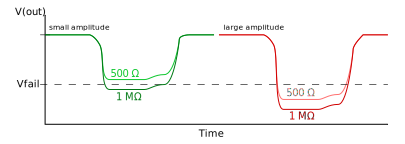
\includegraphics{src/4/figures/zout_impact_time_domain.pdf}
  \caption{Represented impact of output load impedance on the output waveform during a disturbance with a small amplitude (green) and a large amplitude (red)}
  \label{fig:impact-time-domain-load}
\end{figure}

% Conclusion, the main impact is not the characterization load, but the single failure criteria
In conclusion, the load value used during characterization does not seem to be the main source of error.
Rather, it is the consequence of using a single level as failure criteria, which eliminates a lot of information.
Basically, it oversimplifies the waveform of the output.
This is illustrated by figure. \ref{fig:impact-single-failure-criteria}.
Any disturbance under the failure criteria is modeled as no disturbance.
This is the case even if the disturbance is just below the failure criteria, without crossing it.
On the contrary, any disturbance beyond the failure criteria uses the failure level for modeling.
The max value of the output may be much larger than the failure criteria, however, it will still be modeled as a square pulse of amplitude Vfail.

\begin{figure}[!h]
  \centering
  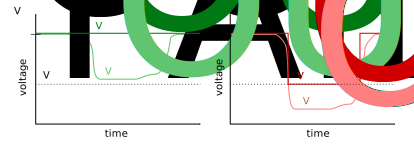
\includegraphics{src/4/figures/bad_output_modelling.pdf}
  \caption{Lack of accuracy caused by the use of a single failure criteria to model the output}
  \label{fig:impact-single-failure-criteria}
\end{figure}

% Talk about static impedances vs dynamic
%TODO: Not studied ?
% Talk about real vs imaginary impedances
%TODO: Not studied

\subsubsection{Other sources}

%TODO: Make section ? Speak about limitations with multiples nets that are responsible for error propagation
%TODO: Limitation with multiple nets. Interactions between inputs. Diamond-like connections

% What was the promise of this model
This method looked rather promising in terms of applicability.
In theory, a block could be characterized once, and its model reused in different places.
The robustness of a full system could be quickly and easily deduced from the models of its parts.

% Real outcome is that it's not working well
However, with the study case exposed earlier, several issues arose that clearly limit the ability of the model to perform as expected.

% Main issue
So far the main issue of this method is to be limited to a binary fail/no fail criteria.
In some cases, the specification could be used to set this criteria, but mostly it was an arbitrary level.
For digital cells, a binary criteria is correct because above a certain input level disturbance an output can be switched, and the failure is then clear.
However, for most analog functions, there is no clear failure.
Most nets will have degraded values until extreme levels where biasing might completely fail.
Sometimes, the product is destroyed before reaching those extreme levels.
In any case, the binary criteria hides a lot of information about the degradation.

% Secondary issue
It was also suspected that the output load used during characterization might impact the results too much.
In practice, it was proven in the case of the regulator that this is not exactly true.
Changing the load can induce a varation, but seemingly more limited than the impact of the binary failure criteria.

% Directivity ?
% Basically : WE ASSUME STRESS AND FAILURES PROPAGATE FROM INPUT TO OUTPUT. MAY NOT BE THE CASE. ALSO, MAY NOT WORK IN REVERSE WITH SINGLE2MANY BLOCK CONNECTIONS

% Next
The next section will explore a modification of the characterization method to fix the binary failure criteria issue.

\subsection{Proposed workaround}
% What's the plan to fix that crap
As it was identified earlier, a binary failure criteria for modeling the output waveform is the main cause of error.
A modification to the characterization method is proposed.

% What is kept in the method, What is modified
The characterization is still performed per-block, still by injecting variable width and variable amplitude rectangular pulses on an input.
However, the failure criteria on the output is now eliminated.
Instead, two values are recorded rather than one.
First, the maximum amplitude value on the output is measured.
Second, the width of the disturbance is also sampled.
It is measured at a fixed percentage of the maximum amplitude.

% What value and why ?
In our current study case, a value of 90\% was employed.
It provides some noise-margin against voltage fluctuations near maximum amplitude during the pulse.
The concept is illustrated in Fig. \ref{fig:impact-single-failure-criteria}.
Basically, this method can be seen as modelling and simplifying a complex waveform into a rectangular waveform.

\begin{figure}[!h]
  \centering
  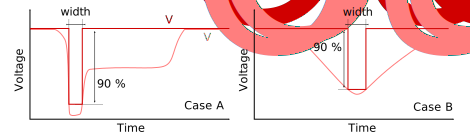
\includegraphics{src/4/figures/better_output_modelling.pdf}
  \caption{Improved output modelling method based on 90\% of maximum disturbance amplitude}
  \label{fig:impact-single-failure-criteria}
\end{figure}

% Result, 2 curves - explain what they are.
Since two parameters are now recorded, two curves are obtained per block rather than one.
The first curve is $out_{amplitude} = f(in_{width}, in_{amplitude})$.
The second curve is $out_{width} = f(in_{width}, in_{amplitude})$.

% What is the improvement
These two curves constitute the model of the block.
Like done previously, models are chained together to deduce the robustness of a complete function.
Fig. \ref{fig:full-method-v2} illustrates the entire characterization and chaining process using these two curves per model.

\begin{figure}[!hp]
  \centering
  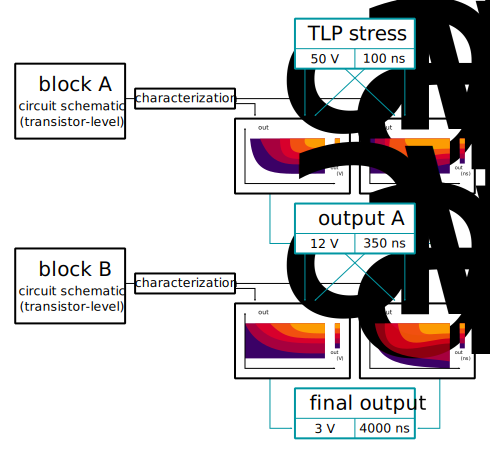
\includegraphics{src/4/figures/full_method_overview_v2.pdf}
  \caption{Overview of improved bottom-up method - example with two blocks}
  \label{fig:full-method-v2}
\end{figure}

% Explain the figure
After each block is characterized, a \gls{tlp} stress is applied to the first model.
In this example, the pulse has an amplitude of 50V ($in_{amplitude}$) and a width of 100ns ($in_{width}$).
The first curve indicates the output is disturbed with a maximum amplitude of 12V ($out_{amplitude}$).
The second curve indicates the output is disturbed during 350ns ($out_{width}$).
These two values can now be applied to the model of block B with the same process.
Finally, it is found that the output is disturbed at a maximum amplitude of 3V during 4000ns.

\subsection{Application to the testchip}

% Apply to the teschip
The new method is applied to the same three blocks of the testchip for checking its validity.
The pre-regulator is characterized first (Figs \ref{fig:pre-reg-cz-v2-amp} and \ref{fig:pre-reg-cz-v2-width}).

\begin{figure}[!h]
  \centering
  \includegraphics[width=0.95\textwidth]{src/4/figures/vpre_cz_V2_amplitude.png}
  \caption{Pre-regulator characterization - $min(V_{out}) = f(V_{in}, W_{in})$}
  \label{fig:pre-reg-cz-v2-amp}
\end{figure}

\begin{figure}[!hp]
  \centering
  \includegraphics[width=0.95\textwidth]{src/4/figures/vpre_cz_V2_width.png}
  \caption{Pre-regulator characterization - $W_{out} = f(V_{in}, W_{in})$}
  \label{fig:pre-reg-cz-v2-width}
\end{figure}

% Detail graph - pre-reg amplitude
Fig. \ref{fig:pre-reg-cz-v2-amp} plots a gradient representing the minimal amplitude of the output signal,
in function on the input stress characteristics (amplitude and width).
The characterized block is the pre-regulator.
It plots the \textbf{minimal} amplitude and not the \textbf{maximal} amplitude because the input stress is negative.
Therefore, a smaller value on the output means a larger disturbance.

% Analysis
It can be noticed that the output voltage is mostly dependent on the input voltage, and not on the input pulse width.

% Detail graph - pre-reg width
Fig. \ref{fig:pre-reg-cz-v2-width} is the second curve obtained by characterizing the pre-regulator.
It plots a gradient representing the disturbance width of the output, in function on the input voltage.
The width of the disturbance is calculed by at 90\% of the minimum output amplitude.

% Analysis
This output width characteristic is quite different from the previous output voltage characteristic.
Here, the output width depends on both the input amplitude and input width.
For input voltages mostly above 2V, the output width does not depend on the input width.
It is exclusively tied to the input voltage.
Then, below 2V, this behavior becomes reversed. The output width is directly dependent on the input width,
no matter the input voltage.
%TODO: Try to explain why

% Summarize
Both Figs. \ref{fig:pre-reg-cz-v2-amp} and \ref{fig:pre-reg-cz-v2-width} constitute the pre-regulator model.

\begin{figure}[!htb]
  \centering
  \includegraphics[width=0.95\textwidth]{src/4/figures/bandgap_cz_V2_amplitude.png}
  \caption{Bandgap characterization - $min(V_{out}) = f(V_{in}, W_{in})$}
  \label{fig:bandgap-cz-v2-amp}
\end{figure}

\begin{figure}[!htb]
  \centering
  \includegraphics[width=0.95\textwidth]{src/4/figures/bandgap_cz_V2_width.png}
  \caption{Bandgap characterization - $W_{out} = f(V_{in}, W_{in})$}
  \label{fig:bandgap-cz-v2-width}
\end{figure}

% Analyse bandgap cz
The bandgap is also characterized with the exact same approach.
The output amplitude curve in Fig. \ref{fig:bandgap-cz-v2-amp} has mostly an input-amplitude dependency, except for large voltage disturbances.
The output width curve in Fig. \ref{fig:bandgap-cz-v2-width} has a clear input voltage and width dependency.
This means the output is disturbed because of an energy level, not just a signal level.

%TODO: Inverse colorscale - small amplitude means more disturbed
\begin{figure}[!htb]
  \centering
  \includegraphics[width=0.95\textwidth]{src/4/figures/regulator_cz_V2_amplitude.png}
  \caption{Regulator characterization - $min(V_{out}) = f(V_{in}, W_{in})$}
  \label{fig:reg-cz-v2-amp}
\end{figure}

%TODO: Fix the colorscale
\begin{figure}[!htb]
  \centering
  \includegraphics[width=0.95\textwidth]{src/4/figures/regulator_cz_V2_width.png}
  \caption{Regulator characterization - $W_{out} = f(V_{in}, W_{in})$}
  \label{fig:reg-cz-v2-width}
\end{figure}

% Analyse regulator cz
Finally, the regulator is also characterized.
The output amplitude curve in Fig. \ref{fig:reg-cz-v2-amp} has a clear input voltage and width dependency.
Therefore, the output voltage is disturbed because of an excedent energy on the input.
A large-amplitude short pulse and a small-amplitude long pulse should the disturb the output almost identically.

The output width curve in Fig. \ref{fig:reg-cz-v2-amp} is the most complex of all to interpretate.
Both voltage and width impact the output.
Beyond an input width of 7500ns, the output is suddenly heavily disturbed.
Just below 7300ns, the curve value is XXXX ns.
At 7500ns, the output width is now XXXXns.
This specific area of the curve looks like a clear soft-failure, where the system suddenly goes into reset or safe-mode, and a long procedure to restart it happens.

% Conclude
%TODO
Input voltage output voltage no direct relation
width also plays a role

% Apply a TLP to the models
